% Part: history
% Chapter: biographies 
% Section: emmy-noether

\documentclass[../../../include/open-logic-section]{subfiles}

\begin{document}

\olfileid{his}{bio}{noe}

\olsection{Emmy Noether}

\begin{figure}[h!] 
\centering 
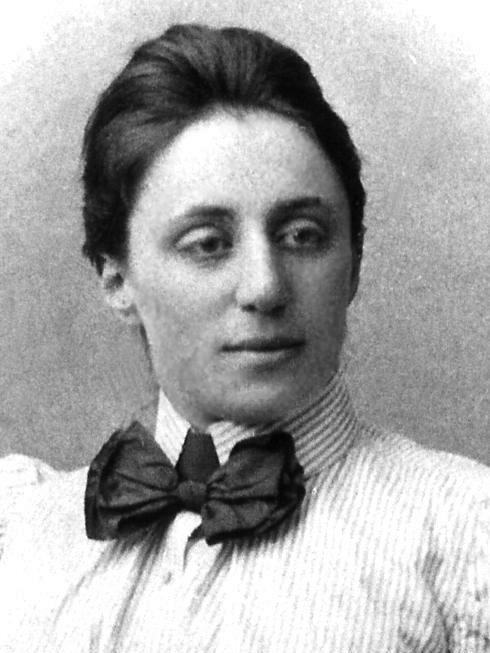
\includegraphics[scale=1.25]{emmy-noether.png}
\caption{Emmy Noether. Photo Credit: Wikimedia Commons.} 
\end{figure}

Emmy
Noether was born in Erlangen, Germany on March 23, 1882, to an upper-middle
class scholarly family. Hailed as the "mother of modern algebra," and
despite the barriers to women's education that were prevalent at the time,
Noether was, and remains to be, a well-respected scholar in both
mathematics and physics. Young girls at the time were meant to be educated
in arts and were not allowed to attend college preperatory schools.
However, after auditing classes at the University of G\"{o}ttingen and the
University of Erlangen, she was finallyable to enrol at Erlangen in 1904
when their policy was updated to allow female students. She recieved her
Ph.D. in mathematics in 1907.

Despite her qualifications, Noether experienced much resistance during her
career. From 1908 - 1915 she taught at Erlangen with no pay. During this
time she caught the attention of David Hilbert, who invited her to
G\"{o}ttingen. However, there was resistance to her coming due to her being
a woman, and she was only able to lecture under Hilbert's name, and with no
pay. During this time she proved what is now known as Noether's theorem,
which is still used in theoretical physics today. Finally, in 1919 Noether
was deemed eligible for tenure, and was finally able to lecutre and take on
PhD students. Her students often noted her complete disregard for
appearance, and her passion for mathematics.

Noether came from a Jewish family, and in 1933, due to the rise of
anti-Semitic government policy in Germany, she was let go from her position
at G\"{o}ttingen. Because of her Jewish heritage and her leftist political
stance, she was forced to leave Germany altogeher. Luckily, Noether was
able to emigrate to the United States for a temporary position at Bryn
Mawr, Pennsylvania. During her time there she also lectured at Princeton,
although she found the univeristy to be unwelcoming to women
\citep[81]{Dick1981}. In 1935 Noether underwent an operation to remove a
uterine tumour. She passed away due to an infection as a result of the
surgery, and was buried at Bryn Mawr.

\begin{reading} 
\begin{itemize} 
\item The Perimeter Institute for
Theoretical Physics has their lectures on Noether's life and influence
available online. See \citet{Perimeter2015}.

\item For a written biography of Noether, see \citet{Dick1981}.

\item If you're tired of reading, \emph{Stuff You Missed in History Class}
has a podcast on Noether's life and influence. See \citet{Frey2015}.

\item The collected works of Noether are available in the original German,
see \citet{Noether1983}. 
\end{itemize} 
\end{reading}

\end{document}
